%%%%%%%%%%%%%%%%%%%%%%%%%%%%%%%%%%%%%%%%%%%%%%%%%%%%%%%%%%%%%%%%%%%%%
%% sec_benchmarks.tex
%% General validation benchmarks for periodic and spin-polarized RT-TDDFT
%%%%%%%%%%%%%%%%%%%%%%%%%%%%%%%%%%%%%%%%%%%%%%%%%%%%%%%%%%%%%%%%%%%%%

\section{Validation of Periodic and Spin-Polarized RT-TDDFT}
\label{sec:results}

We first validate the periodic and spin-polarized RT-TDDFT
implementation in \texttt{RMG} by comparing current-derived optical
spectra with independent real-time calculations performed with
\texttt{Octopus}, an established real-space RT-TDDFT code for finite
and extended systems.\cite{octopus-2020}  The benchmark set was chosen
as a progression of increasing complexity: a one-dimensional periodic
hydrogen-dimer reference, pristine monolayer hBN, bulk Si, and
spin-polarized \ch{CrI3}.  The purpose of these comparisons is not to
establish quantitatively normalized optical conductivities or
dielectric functions, but to test whether RMG reproduces the principal
spectral features obtained from an independent RT-TDDFT implementation
at a comparable semilocal-DFT level.  Accordingly,
Fig.~\ref{fig:benchmarks} reports optical spectra in arbitrary units
and the comparison emphasizes peak positions, dominant spectral
structures, overall spectral envelopes, and polarization or spin
dependence where applicable.

\begin{figure}[ht!]
  \centering
  \begin{tabular}{@{}cc@{}}
    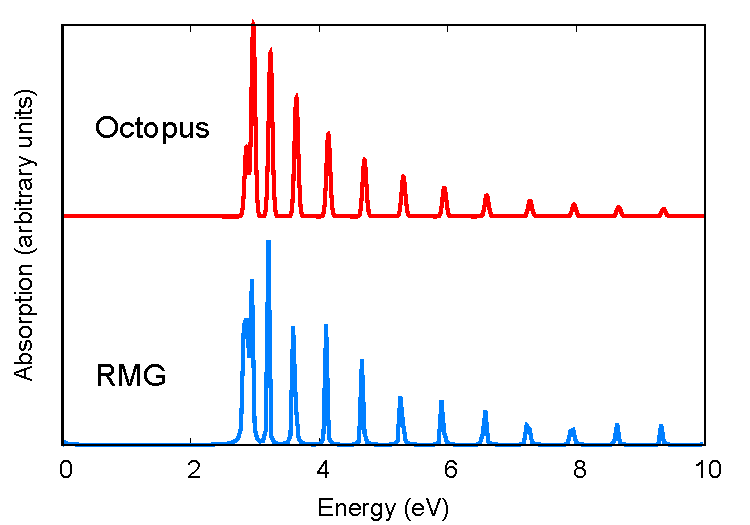
\includegraphics[width=0.48\columnwidth]{Figs/out-h2.pdf} &
    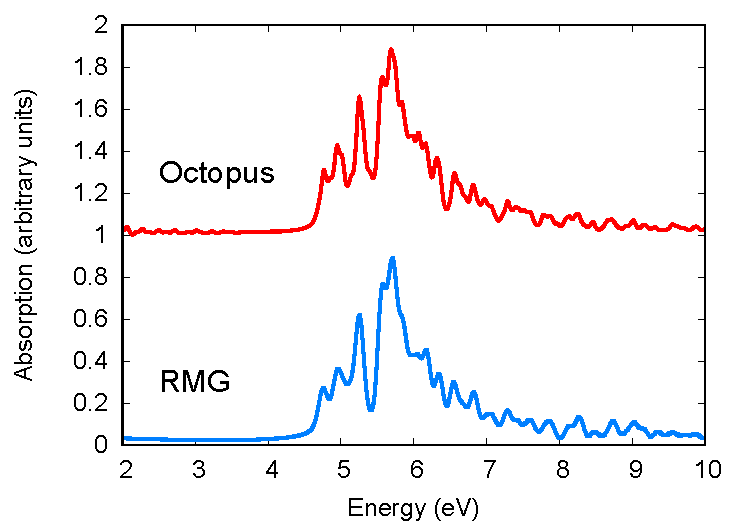
\includegraphics[width=0.48\columnwidth]{Figs/out-hBN.pdf} \\
    (a) & (b) \\
    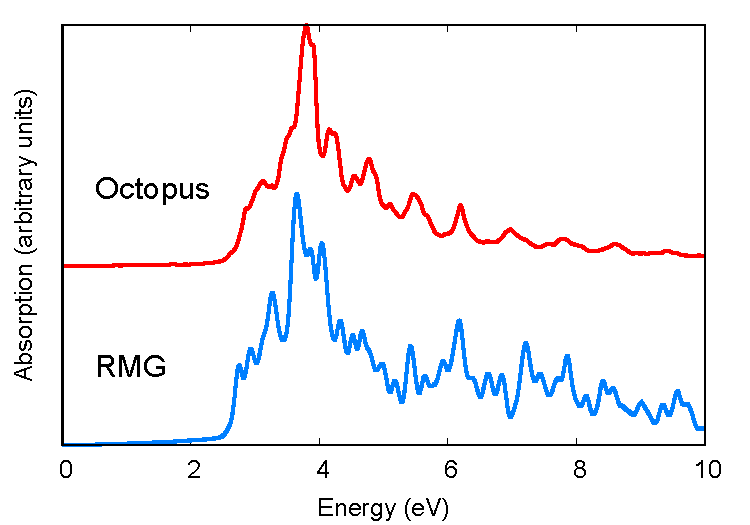
\includegraphics[width=0.48\columnwidth]{Figs/out-Si.pdf} &
    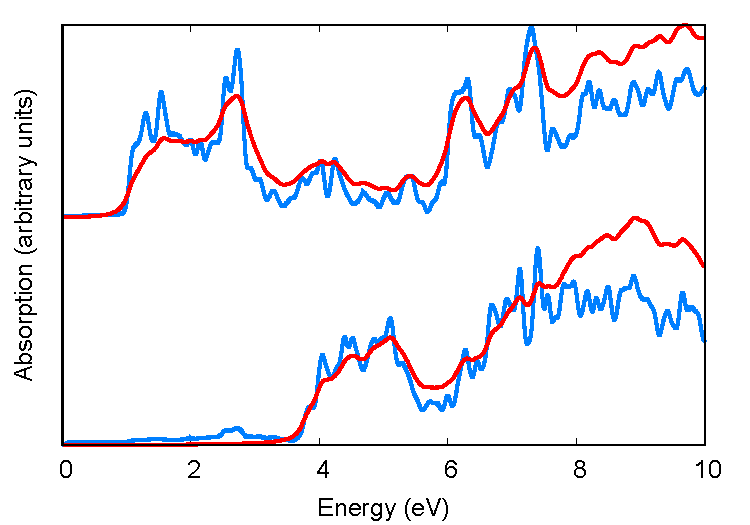
\includegraphics[width=0.48\columnwidth]{Figs/out-CrI3.pdf} \\
    (c) & (d)
  \end{tabular}
  % CHECK WITH LIANGBO: confirm Octopus provenance and comparable PBE-level settings for all four benchmark reference curves.
  \caption{\footnotesize
    Optical spectra in arbitrary units from periodic RT-TDDFT
    calculations with \texttt{RMG} and independent \texttt{Octopus}
    reference calculations for systems of increasing complexity:
    (a) a one-dimensional periodic hydrogen-dimer reference,
    (b) pristine monolayer hBN, (c) bulk Si, and
    (d) spin-polarized \ch{CrI3}.  The comparison emphasizes peak
    positions and dominant spectral features rather than absolute
    intensity.
  }
  \label{fig:benchmarks}
\end{figure}

The one-dimensional hydrogen-dimer system provides the simplest
periodic reference.  The model consists of hydrogen dimers repeated
along one lattice direction with large transverse vacuum, and therefore
tests the basic k-resolved propagation and current-response machinery
without the additional complications of a multidimensional crystal.
RMG reproduces the sequence of major peaks obtained from the
\texttt{Octopus} calculation over the plotted energy range, providing
a basic cross-code validation of the periodic propagation and
current-response implementation.

Pristine monolayer hBN provides a genuinely two-dimensional periodic
benchmark.  The RMG calculation uses a non-spin-polarized monolayer
slab with vacuum normal to the layer and dense in-plane k-point
sampling.  Similar monolayer hBN tests have been used in recent
periodic velocity-gauge RT-TDDFT implementation
work.\cite{Hanasaki-2023}  The RMG and \texttt{Octopus} spectra show
a similar low-energy onset and similar dominant structures in the main
spectral envelope, validating the two-dimensional periodic
implementation and the in-plane current response for an insulating
material.  As expected for semilocal PBE-level calculations, this
benchmark should not be interpreted as a quantitative description of
the strongly excitonic experimental optical spectrum of
low-dimensional BN materials, where long-range electron-hole
interactions are known to be important.\cite{Wirtz-BN-excitons-2006}
Detailed spin-polarized RT-TDDFT applications to hBN color centers are
treated separately in a companion study.
% TODO: add citation to Liangbo companion hBN manuscript when bibliographic status is set.

Bulk Si then tests the full three-dimensional periodic implementation,
including dense k-point sampling and the complex matrix path required
away from $\Gamma$.  The spectra from RMG and \texttt{Octopus} show
similar low-energy behavior and reproduce the dominant structure in
the approximately 3--4 eV region, while somewhat larger differences
are visible in the higher-energy fine structure.  This level of
agreement is consistent with the role of Si as a standard benchmark
for periodic velocity-gauge RT-TDDFT
implementations.\cite{Hekele-2021}

Finally, \ch{CrI3} provides the most demanding member of the general
benchmark set: a spin-polarized periodic calculation including DFT+U
for the Cr $3d$ states.  The available RMG input is collinear
spin-polarized and includes a $U=3.0$ eV correction for the Cr $3d$
states.  The comparison in Fig.~\ref{fig:benchmarks} shows that RMG
captures the main spectral structures obtained in the independent
calculation for this magnetic material.  We interpret this benchmark
as a test of the spin-polarized periodic RT-TDDFT workflow, not as a
complete treatment of spin-orbit-coupled or excitonic
magneto-optical physics in \ch{CrI3}, which requires physics beyond
the present collinear PBE+U-level
workflow.\cite{Wu-CrI3-excitons-2019}

Taken together, these four benchmarks show that the RMG implementation
reproduces the principal spectral features of an independent RT-TDDFT
code across one-dimensional, two-dimensional, three-dimensional, and
spin-polarized periodic systems.  The following NV$^{-}$-center
calculations provide an additional physics-specific validation layer by
testing defect orbital character, polarization selection rules,
spin-channel selectivity, active-space convergence, and supercell-size
effects in large diamond supercells.
